\chapter{Évolution du cahier des charges}
\label{chapter1}

Plusieurs éléments du cahier des charges ont été amenés à changer depuis la première revue de projet.

\section{Nécessité du traçage d'astre}

Le traçage d'astre, vu au départ comme une fonctionnalité intéressante, s'est imposé comme une fonctionnalité nécessaire. En effet il peut être particulièrement difficile pour une personne non initiée à l'astronomie de positionner le télescope vers un astre précis ou de reconnaître un astre que l'on observe. Il nous est donc apparu primordial que le télescope permette d'affranchir l'utilisateur de la nécessité d'avoir des bases en astronomie pour observer le ciel.

\vspace{1cm}

En étudiant les solutions disponibles nous avons trouvé des logiciels de simulation du ciel, comme par exemple le logiciel libre Stellarium.

\begin{figure}[H]
    \centering
    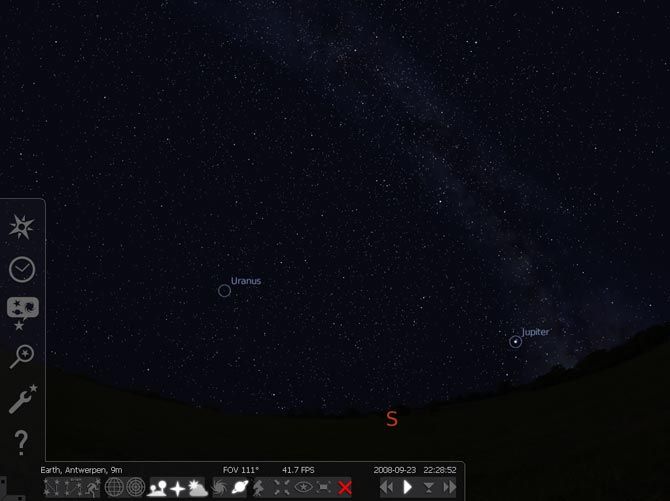
\includegraphics[width=0.49\linewidth]{\figures/photo_stellarium_1.jpg}
	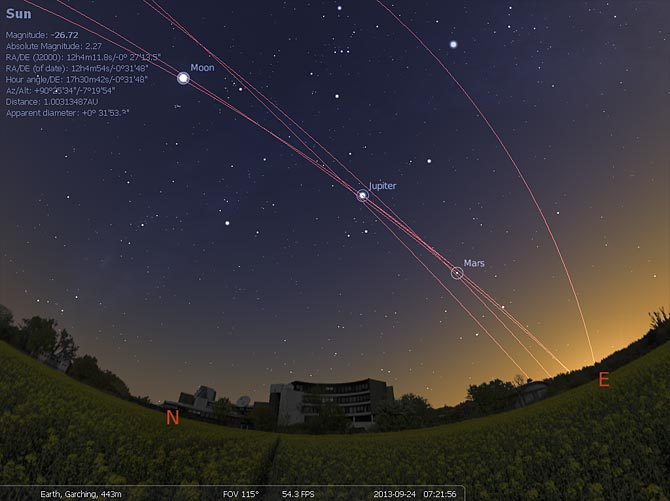
\includegraphics[width=0.49\linewidth]{\figures/photo_stellarium_2.jpg}
    \decoRule
    \caption[
    Captures d'écran de Stellarium]{
    Captures d'écran de Stellarium}
    \label{fig:Captures d'écran de Stellarium}
    \end{figure}

\vspace{1cm}

Celui-ci permet notamment~:
\begin{itemize}[label=$\bullet$]
	\item De connaître les coordonnées d'un astre par rapport à l'endroit sur terre où se situe l'observateur.
	\item De s'orienter dans le ciel selon des coordonnées.
	\item De s'interfacer avec d'autres systèmes logiciels et/ou matériels
	\end{itemize}

Nous avons donc décidé dans un premier temps de développer une interface pour piloter le télescope depuis un ordinateur distant doté de Stellarium. Puis éventuellement d'embarquer Stellarium dans l'ordinateur du télescope. Ainsi Stellarium fera partie intégrante de son interface utilisateur.

Celle-ci pourrait être alors un menu discret permettant de passer de l'exploration virtuelle du ciel à la vue correspondante à travers le télescope à d'autres élément comme un dispositif d'amélioration de la qualité des images prises.

\section{Nécessité d'une centrale inertielle et d'un GPS}

L'utilisation d'un logiciel de traçage d'astre tel Stellarium nécessite la compatibilité du télescope avec les coordonnées d'azimut et d'élévation couramment utilisées en astronomie. Il est également nécessaire pour cela de savoir de quel endroit sur terre le télescope observe le ciel, d'où l'utilisation d'un GPS.

\vspace{1cm}

Pour connaître l'azimut et l'élévation, il faut avoir des repère dans les deux dimensions. Un magnétomètre permet de déterminer la direction du nord et un accéléromètre permet de connaître la direction du sol, c'est à dire la verticale.

Une centrale inertielle est un composant intégrant un magnétomètre, un accéléromètre et un gyroscope. Elle permet de connaître directement les coordonnées absolues de son orientation dans l'espace.

\section{Changement de SoC}

L'utilisation de Stellarium requiert au minimum $512MiB$ de RAM et $1GiB$ pour une utilisation optimale. Or la carte PICO-PI ne dispose que de $512MiB$ de RAM, elle est donc incapable de faire fonctionner Stellarium correctement.

\vspace{1cm}

Nous avons choisi une Raspberry Pi 3 avec $2GiB$ de RAM en remplacement. En dépit de ses faibles capacités d'industrialisations, la Raspberry Pi a l'avantage d'être populaire dans le milieu de l'électronique amateur, c'est-à-dire le publique le plus susceptible d'être intéressé par ce genre de projet.

\vspace{1cm}

La caméra et l'écran utilisés ne seront donc plus ceux fournis avec la PICO-PI mais ceux de la Raspberry Pi, à savoir~:
\begin{itemize}[label=$\bullet$]
	\item Le module Raspicam v2.1 intégrant une caméra IMX219 de $8Mpx$.
	\end{itemize}

L'écran demeure toutefois une option, celui-ci sera intégré si le télescope embarque Stellarium.


